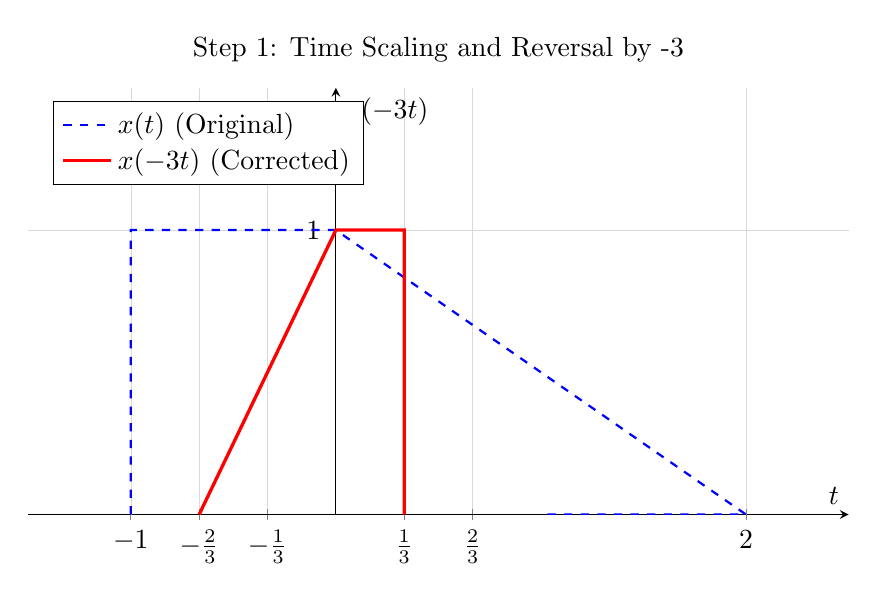
\begin{tikzpicture}
	\begin{axis}[
		% Set the overall style
		width=12cm,
		height=7cm,
		% Title and labels
		title={Step 1: Time Scaling and Reversal by -3},
		xlabel={$t$},
		ylabel={$x(-3t)$},
		% Position axes at the origin
		axis lines=middle,
		% Set axis limits for good spacing
		xmin=-1.5, xmax=2.5,
		ymin=0, ymax=1.5,
		% Set ticks at key fractional and integer points
		xtick={-2/3, -1/3, 0, 1/3, 2/3},
		% Use LaTeX to display tick labels as fractions
		xticklabels={$-\frac{2}{3}$, $-\frac{1}{3}$, $0$, $\frac{1}{3}$, $\frac{2}{3}$},
		ytick={1},
		% --- ADDED LINE ---
		% Add ticks for the original signal's key points
		extra x ticks={-1, 2},
		% --- END ADDED LINE ---
		% Add a grid
		grid=major,
		grid style={line width=.1pt, draw=gray!30},
		% Position the legend
		legend pos=north west,
		legend cell align={left},
		]
		
		% Plot the original signal (dashed blue)
		\addplot[blue, dashed, thick] coordinates {
			(-1,0) (-1,0) (-1,1) (0,1) (2,0) (1,0)
		};
		\addlegendentry{$x(t)$ (Original)};
		
		% Plot the CORRECT scaled and reversed signal (solid red)
		\addplot[red, very thick] coordinates {
			(-2/3, 0) (0, 1) (1/3, 1) (1/3, 0)
		};
		\addlegendentry{$x(-3t)$ (Corrected)};
	\end{axis}
\end{tikzpicture}